
\clearpage
\section{Weight Decay's Mechanistic Effects on Model Behavior}
\label{app:further-wd-analy}



\subsection{Model representations}
\label{app:lin-probe}






\begin{center}
    \textbf{\llamazeropointfiveB{}}\par\smallskip
    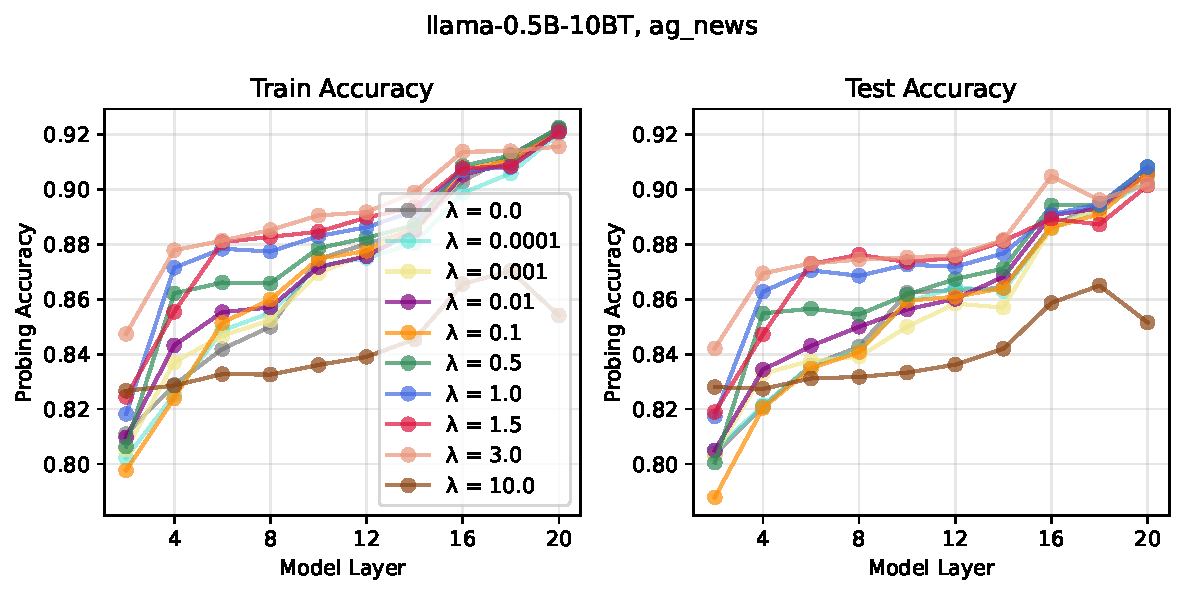
\includegraphics[width=0.32\linewidth, trim={0 0 0 10mm}, clip]{figs/a05_linear_probing/appendix/singlemodel_ag_news_llama-0.5B-10BT.pdf}
    \hfill
    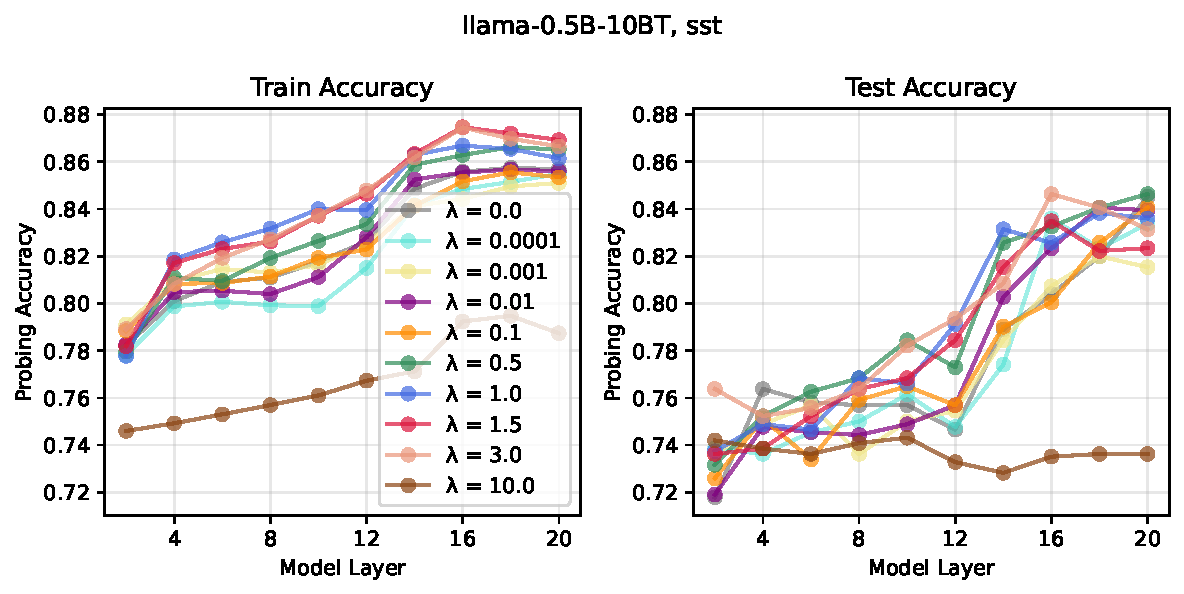
\includegraphics[width=0.32\linewidth, trim={0 0 0 10mm}, clip]{figs/a05_linear_probing/appendix/singlemodel_sst_llama-0.5B-10BT.pdf}
    \hfill
    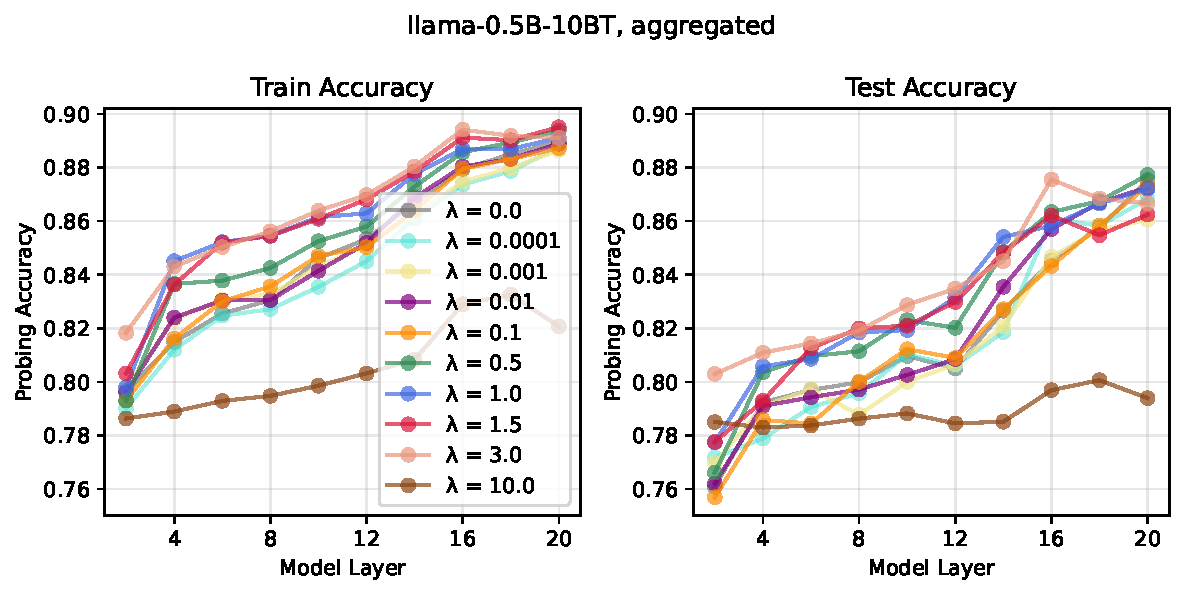
\includegraphics[width=0.32\linewidth, trim={0 0 0 10mm}, clip]{figs/a05_linear_probing/appendix/singlemodel_aggregated_llama-0.5B-10BT.pdf}

    \smallskip
    \textbf{\llamaoneB{}}\par\smallskip
    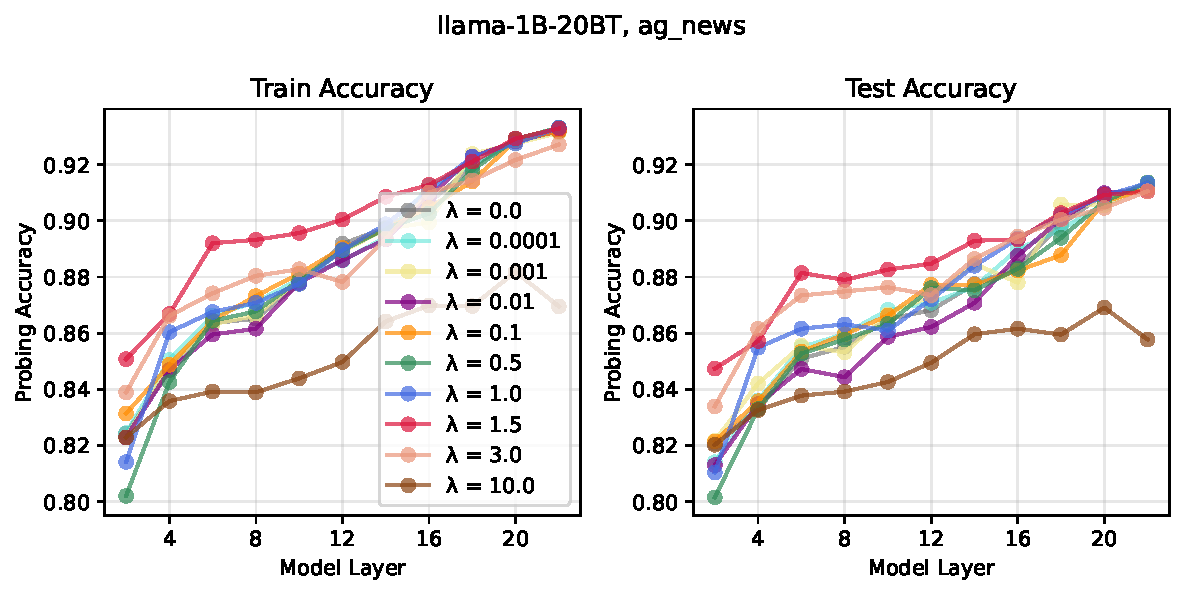
\includegraphics[width=0.32\linewidth, trim={0 0 0 10mm}, clip]{figs/a05_linear_probing/appendix/singlemodel_ag_news_llama-1B-20BT.pdf}
    \hfill
    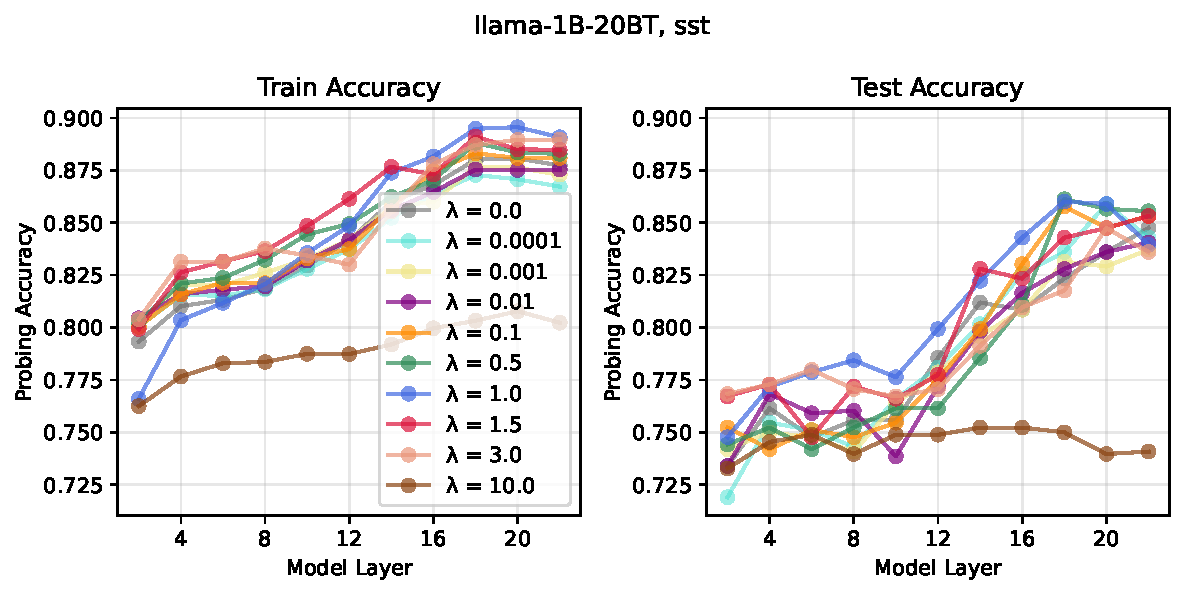
\includegraphics[width=0.32\linewidth, trim={0 0 0 10mm}, clip]{figs/a05_linear_probing/appendix/singlemodel_sst_llama-1B-20BT.pdf}
    \hfill
    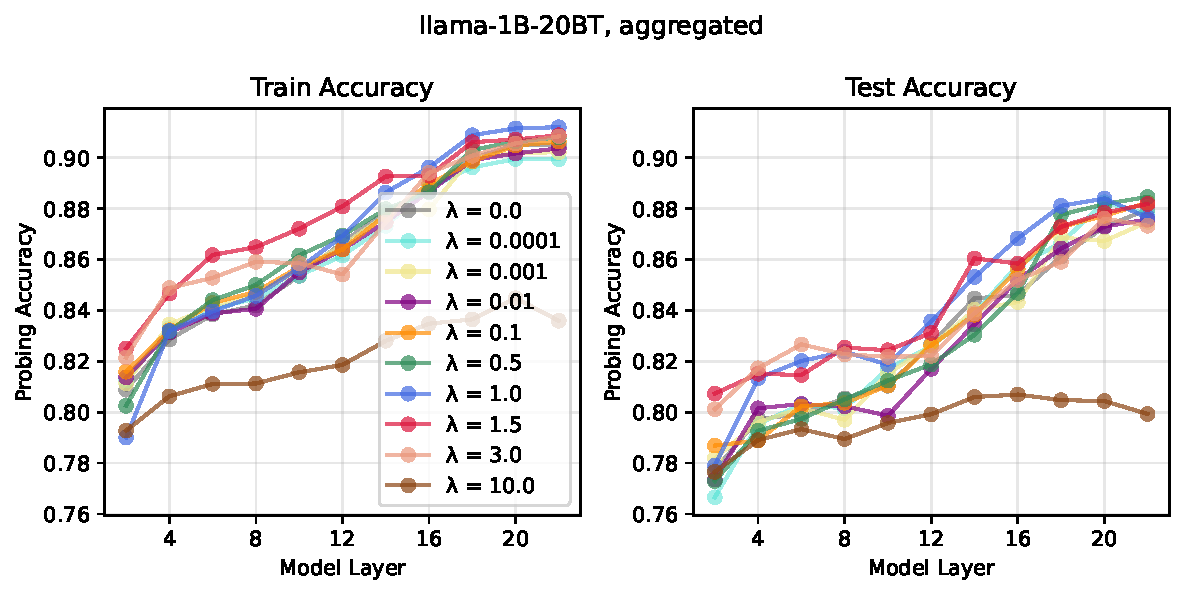
\includegraphics[width=0.32\linewidth, trim={0 0 0 10mm}, clip]{figs/a05_linear_probing/appendix/singlemodel_aggregated_llama-1B-20BT.pdf}

    \smallskip
    \textbf{\llamafourB{}}\par\smallskip
    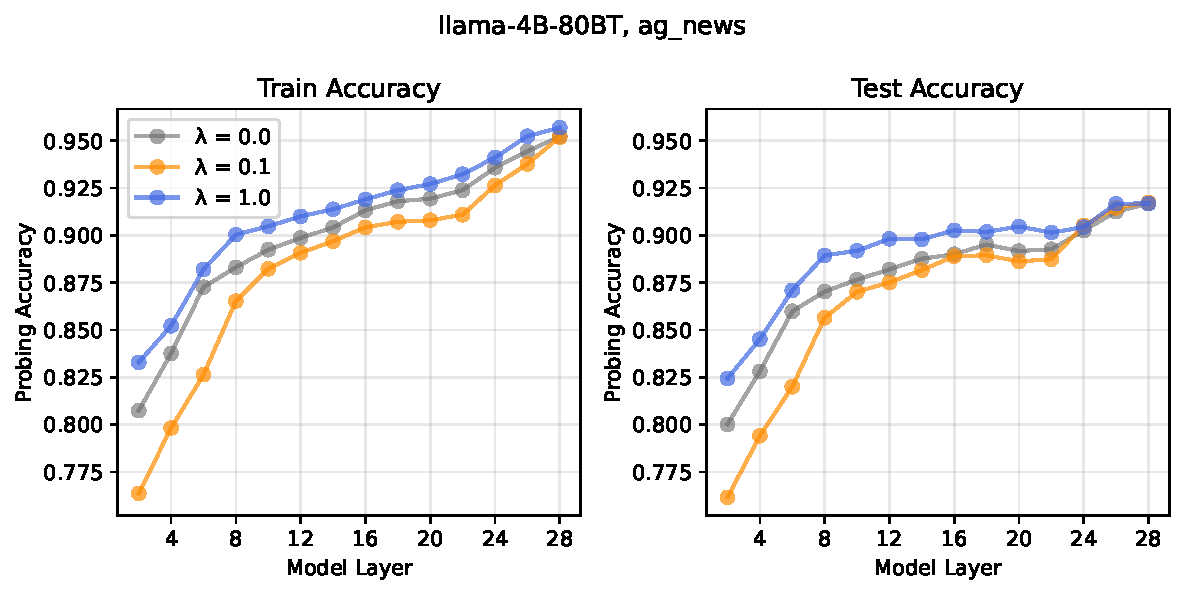
\includegraphics[width=0.32\linewidth, trim={0 0 0 10mm}, clip]{figs/a05_linear_probing/appendix/singlemodel_ag_news_llama-4B-80BT.pdf}
    \hfill
    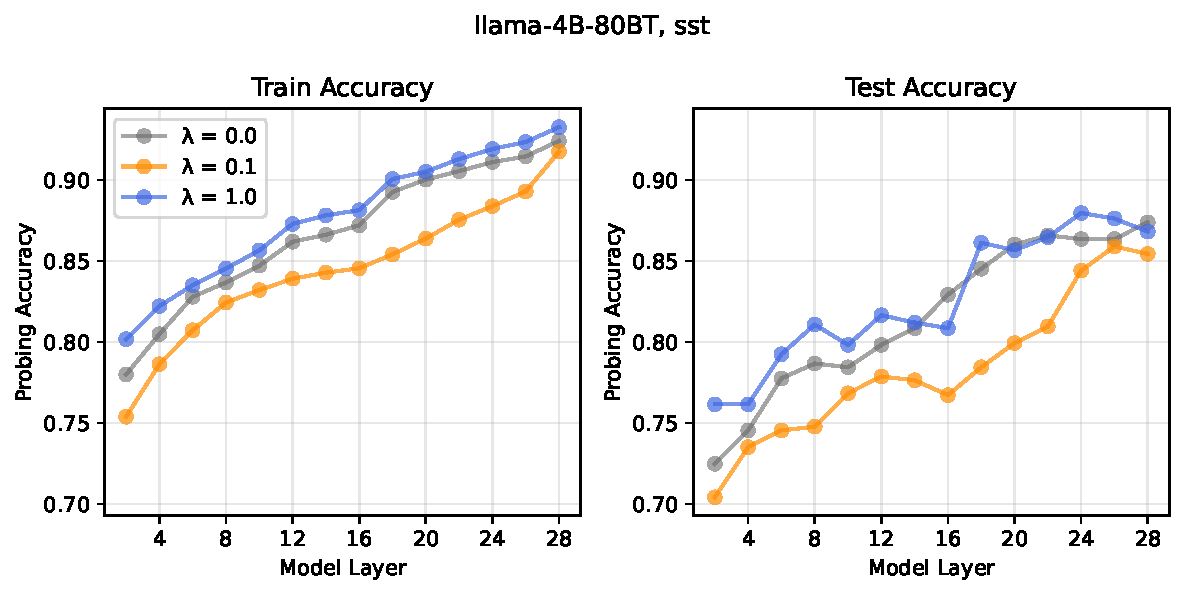
\includegraphics[width=0.32\linewidth, trim={0 0 0 10mm}, clip]{figs/a05_linear_probing/appendix/singlemodel_sst_llama-4B-80BT.pdf}
    \hfill
    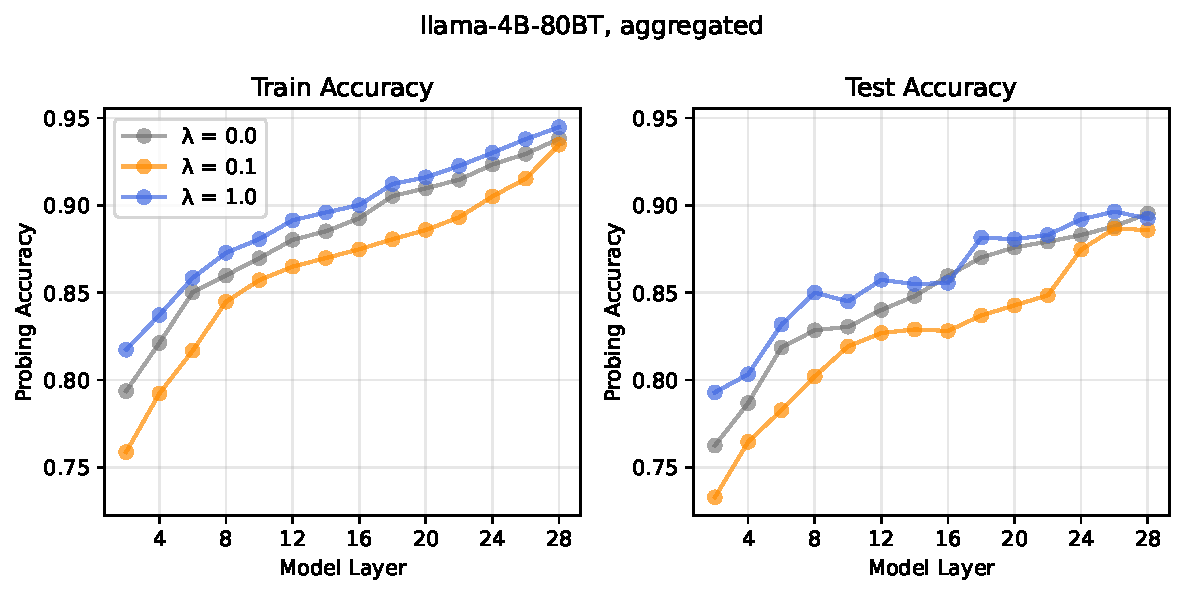
\includegraphics[width=0.32\linewidth, trim={0 0 0 10mm}, clip]{figs/a05_linear_probing/appendix/singlemodel_aggregated_llama-4B-80BT.pdf}

    \smallskip
    \textbf{\olmoonex{}}\par\smallskip
    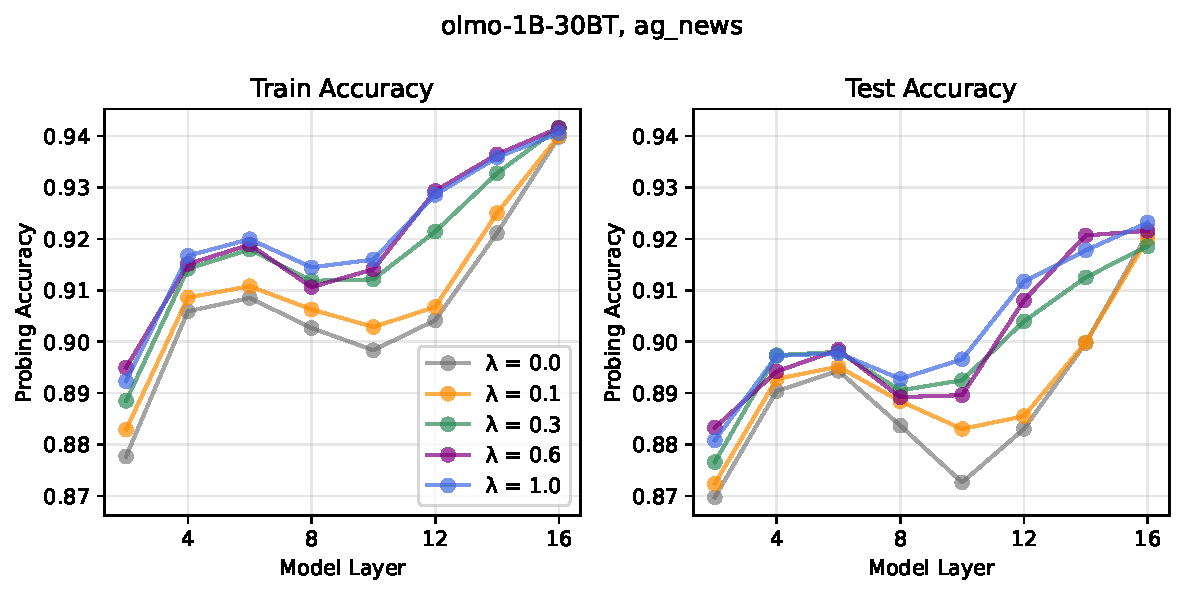
\includegraphics[width=0.32\linewidth, trim={0 0 0 10mm}, clip]{figs/a05_linear_probing/appendix/singlemodel_ag_news_olmo-1B-30BT.pdf}
    \hfill
    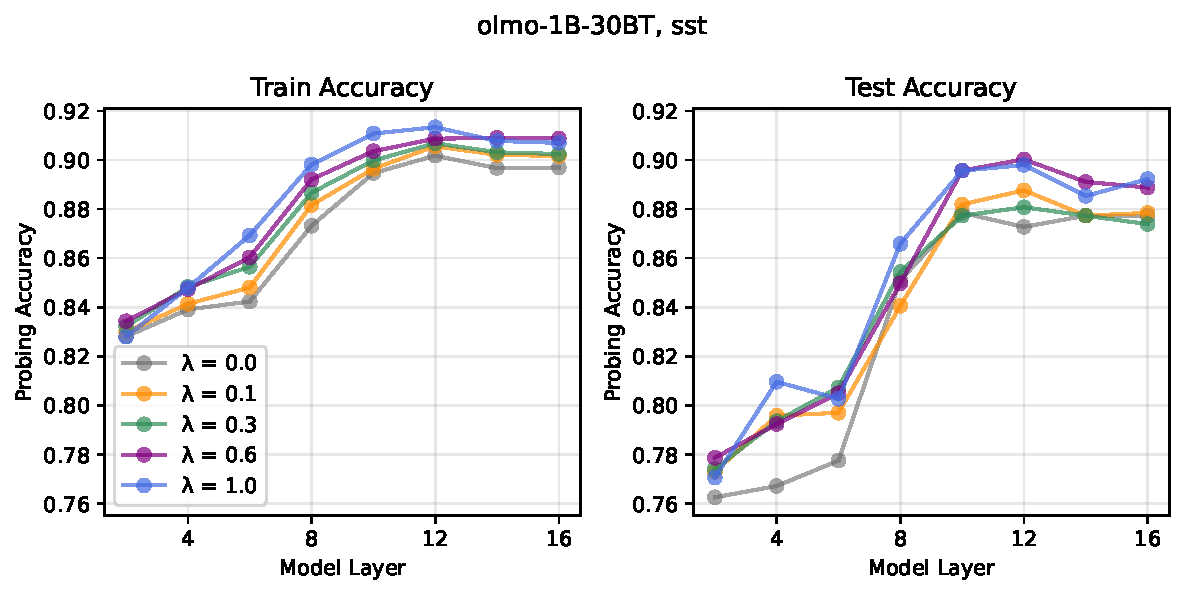
\includegraphics[width=0.32\linewidth, trim={0 0 0 10mm}, clip]{figs/a05_linear_probing/appendix/singlemodel_sst_olmo-1B-30BT.pdf}
    \hfill
    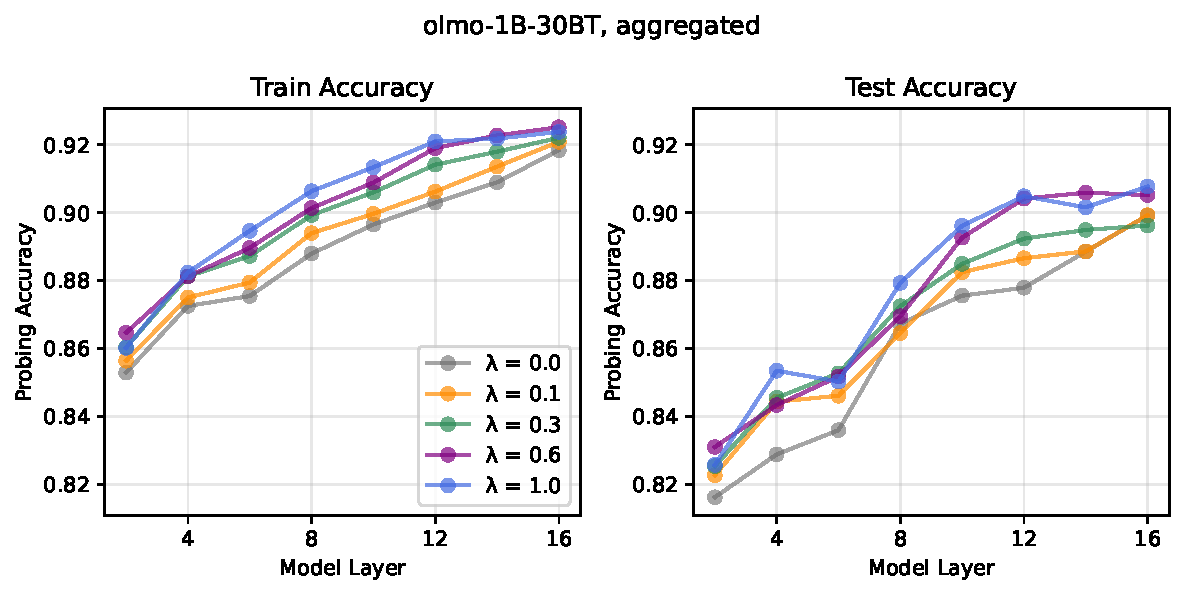
\includegraphics[width=0.32\linewidth, trim={0 0 0 10mm}, clip]{figs/a05_linear_probing/appendix/singlemodel_aggregated_olmo-1B-30BT.pdf}

    \smallskip
    \textbf{\olmosevenx{}}\par\smallskip
    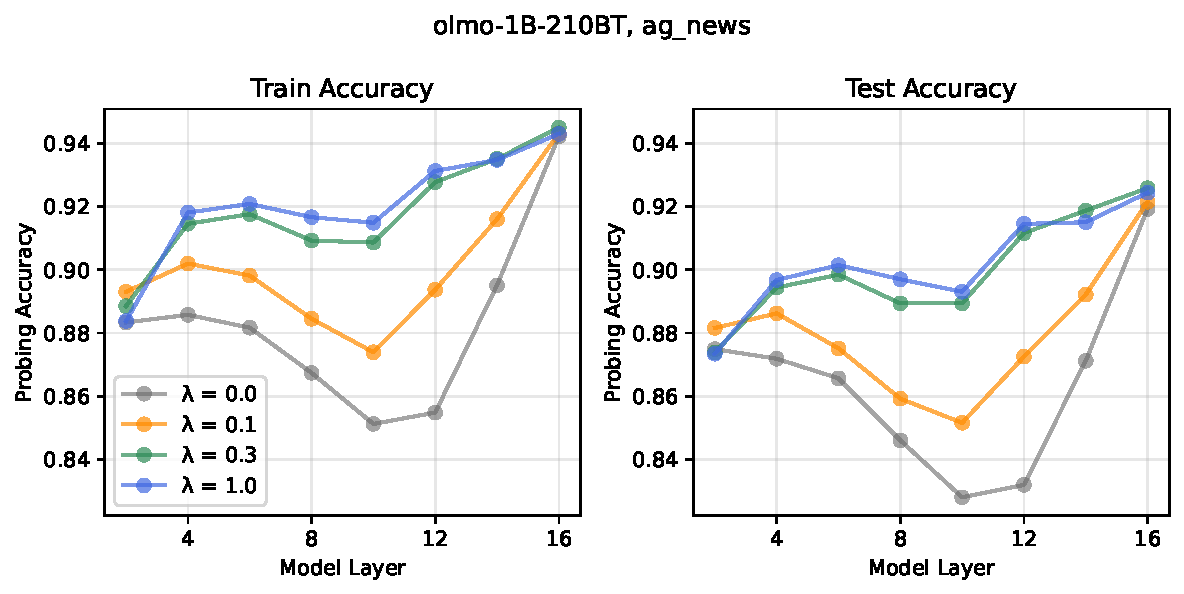
\includegraphics[width=0.32\linewidth, trim={0 0 0 10mm}, clip]{figs/a05_linear_probing/appendix/singlemodel_ag_news_olmo-1B-210BT.pdf}
    \hfill
    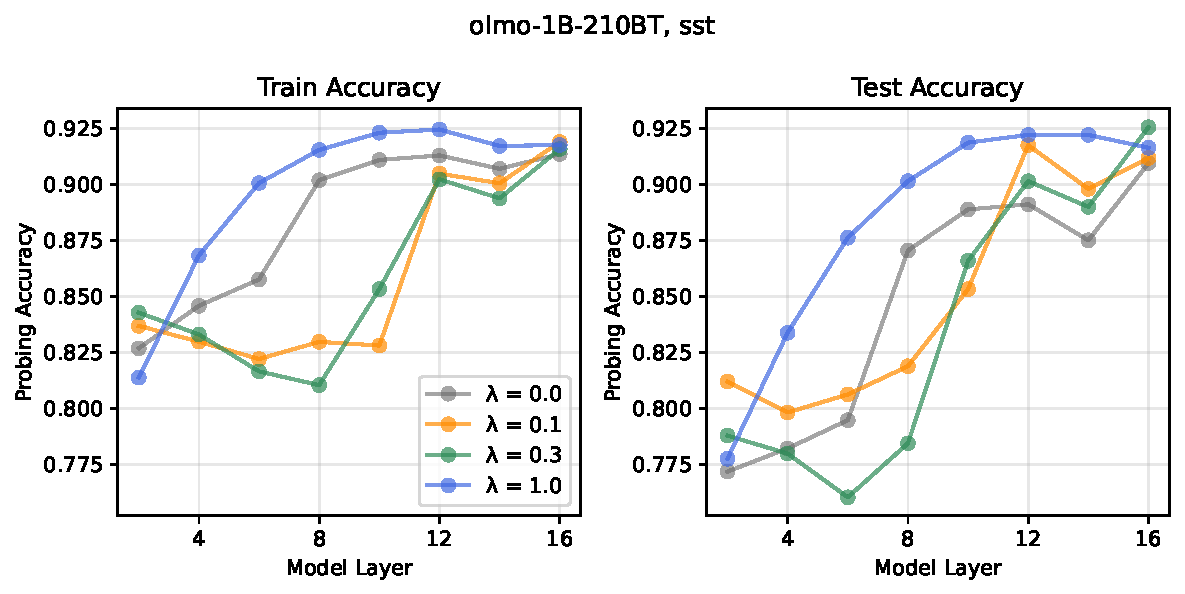
\includegraphics[width=0.32\linewidth, trim={0 0 0 10mm}, clip]{figs/a05_linear_probing/appendix/singlemodel_sst_olmo-1B-210BT.pdf}
    \hfill
    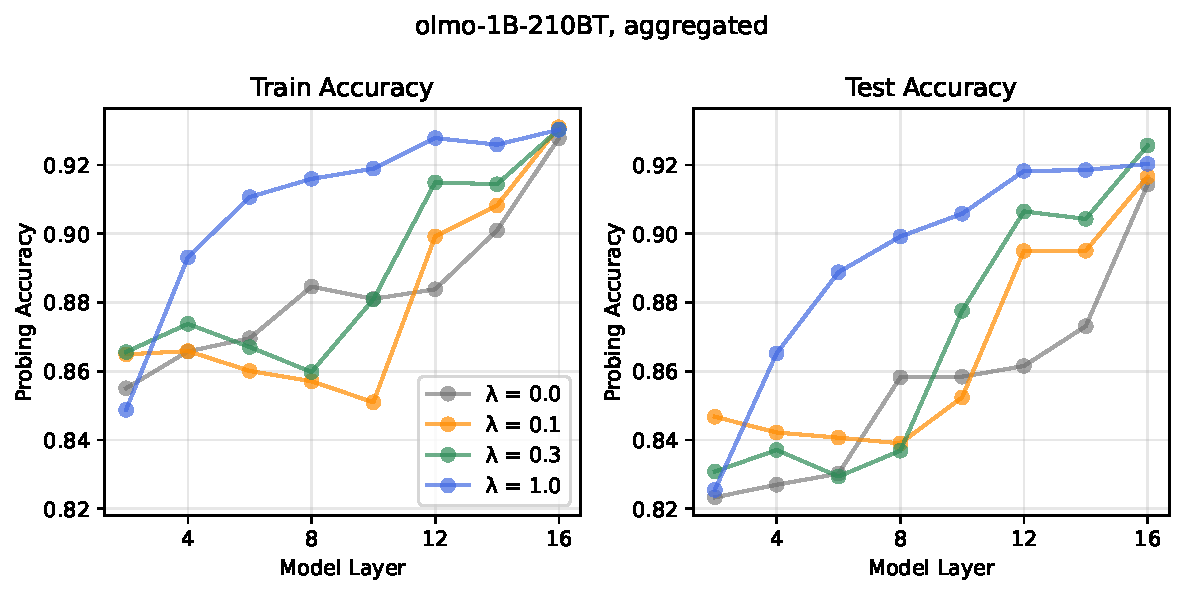
\includegraphics[width=0.32\linewidth, trim={0 0 0 10mm}, clip]{figs/a05_linear_probing/appendix/singlemodel_aggregated_olmo-1B-210BT.pdf}

    \textbf{\hspace{1cm} AG News \hspace{4.7cm} SST \hspace{3.5cm} Average over datasets}\par\medskip
    \captionof{figure}{{\bf Linear probing experiments.} The left two columns, middle two columns, and right two columns show the train and test performance of the linear probes on the SST dataset, on the AG News dataset, and averaged over the two datasets, respectively.}
\end{center}













\begin{figure}[h] 
    \centering
    \begin{subfigure}[b]{\textwidth} 
        \centering
        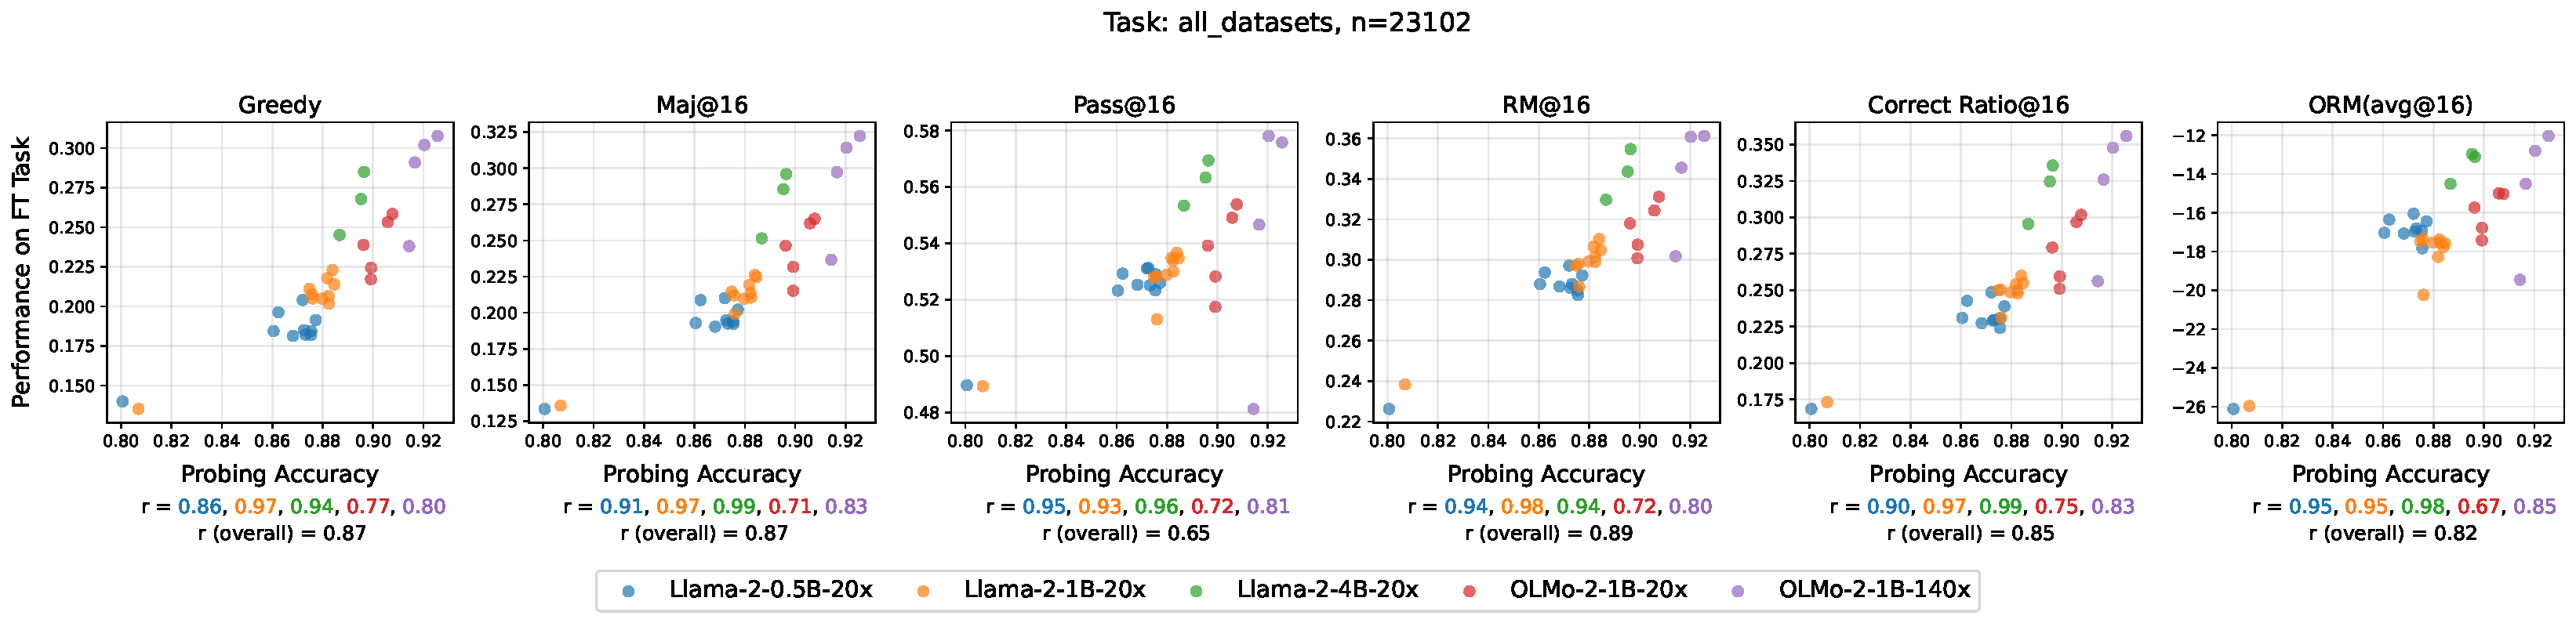
\includegraphics[width=\linewidth, trim={0 0 0 20mm}, clip]{figs/a05b_linear_probing_vs_ft_perf/probe_acc_vs_ft_perf.pdf}
    \end{subfigure}
    \caption{{\bf Probing accuracy is highly predictive of downstream model performance.} The x-axis is the best average probing accuracy of the model (highest probing accuracy out of all model layers). The y-axis the average accuracy of the model over all tasks after fine-tuning. Pretrained models with higher probing accuracies from the linear probing experiments tend to perform better downstream after fine-tuning.} 
    \label{fig:app-probeacc-vs-ftperf}
\end{figure}



\subsection{Attention matrix rank}
\label{app:attention_rank}

\subsubsection{Attention Pseudo-Rank Computation}
\label{app:pseudo_rank}

To quantify the effective dimensionality of weight matrices, we follow \citet{kobayashi2024wdlowrank} and compute the pseudo-rank of the matrices. For a matrix $W$ with singular values $\sigma_1 \ge \sigma_2 \ge \dots \ge \sigma_n$, the pseudo-rank is defined as the ratio $k/n$, where $k$ is the smallest integer satisfying:

\begin{equation}
    \frac{\sum_{i=1}^{k} \sigma_i}{\sum_{i=1}^{n} \sigma_i} \ge 0.95
\end{equation}

This metric represents the fraction of the largest singular values required to capture at least 95\% of the sum of all singular values. In our analysis, we apply this computation to the product of the key-query matrices ($W_{QK} = W_K^T W_Q$) and the value-projection matrices ($W_{VP} = W_P W_V$) to monitor the emergence of low-rank structures during training.



\subsubsection{Additional analyses on attention matrix rank}

\begin{figure*}[h] 
    \centering
    \begin{subfigure}[b]{0.24\textwidth} 
        \centering
        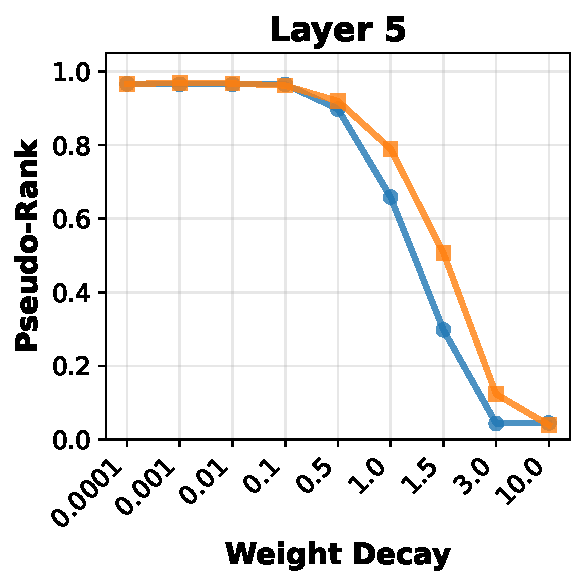
\includegraphics[width=\linewidth]{figs/rank_attn_matrices/llama_layer5_qk.pdf} 
        \caption{Query-Key}
    \end{subfigure}
    \hfill
    \begin{subfigure}[b]{0.24\textwidth} 
        \centering
        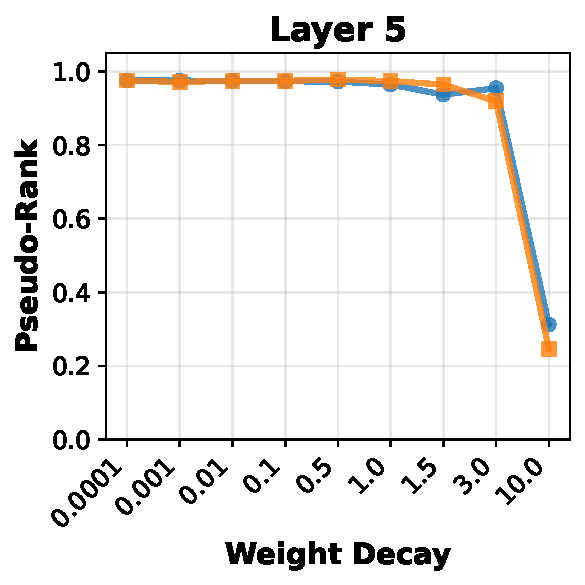
\includegraphics[width=\linewidth]{figs/rank_attn_matrices/llama_layer5_vp.pdf} 
        \caption{Value-Projection}
    \end{subfigure}
    \hfill
    \begin{subfigure}[b]{0.24\textwidth} 
        \centering
        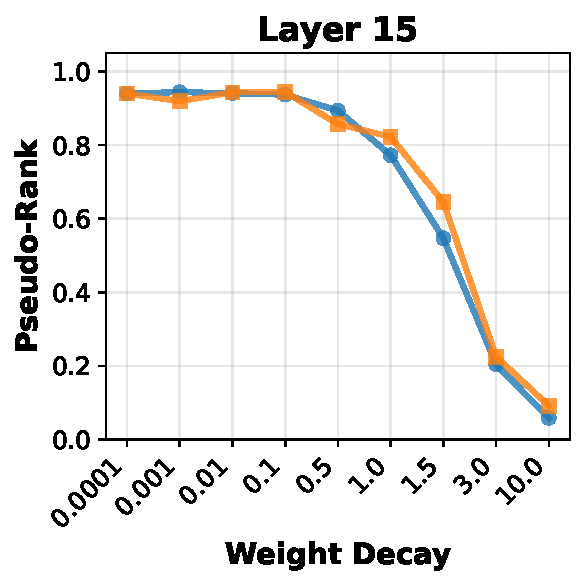
\includegraphics[width=\linewidth]{figs/rank_attn_matrices/llama_layer15_qk.pdf} 
        \caption{Query-Key}
    \end{subfigure}
    \hfill
    \begin{subfigure}[b]{0.24\textwidth}
        \centering
        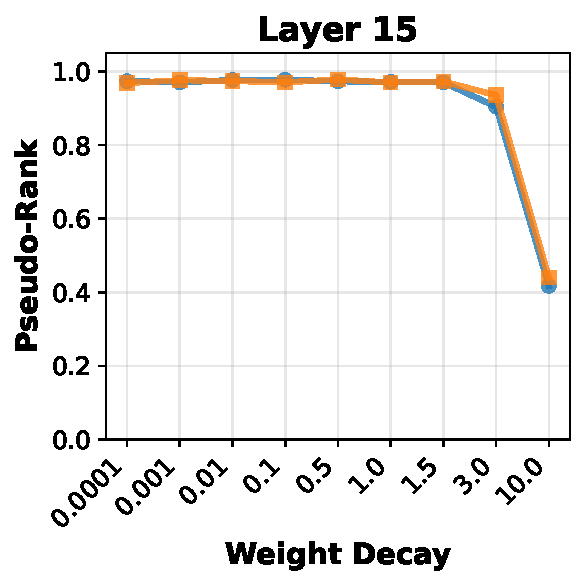
\includegraphics[width=\linewidth]{figs/rank_attn_matrices/llama_layer15_vp.pdf} 
        \caption{Value-Projection}
    \end{subfigure}
    
\includegraphics[width=0.3\textwidth]{figs/rank_attn_matrices/llama_legend.pdf}
    \caption{{\bf Weight decay reduces the rank of attention matrices.} The figure depicts the average pseudo-rank (Appendix~\ref{app:pseudo_rank}) of the query-key ($W_{QK}$) and value projection ($W_{VP}$) matrices in layers 5 and 15 of the fully-trained Llama-2 models at 20 TPP.}
    \label{fig:attention_rank_llama}
\end{figure*}

\begin{figure*}[h] 
    \centering
    \begin{subfigure}[b]{0.4\textwidth} 
        \centering
        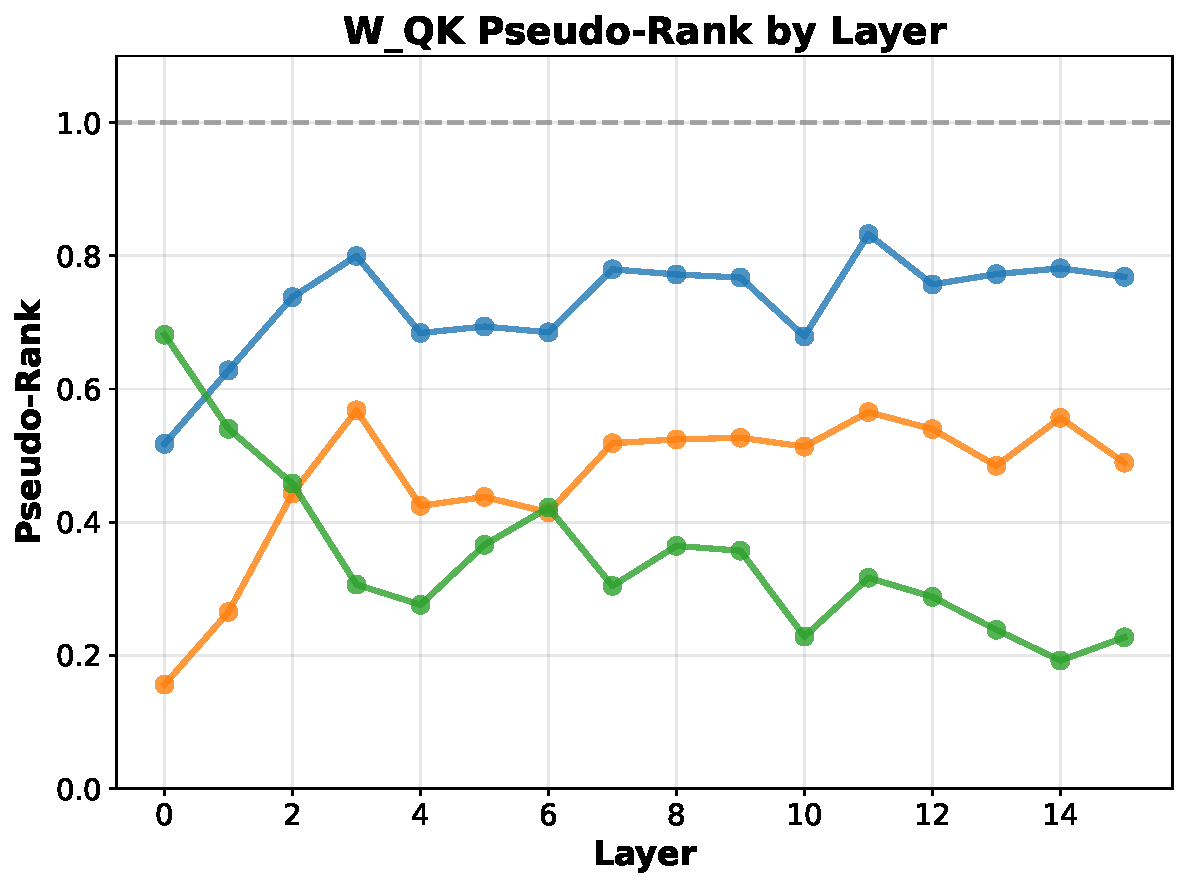
\includegraphics[width=\linewidth]{figs/rank_attn_matrices/olmo2_1b_7x_weight_decay_comparison_qk.pdf} 
        \caption{Query-Key}
    \end{subfigure}
    \begin{subfigure}[b]{0.4\textwidth} 
        \centering
        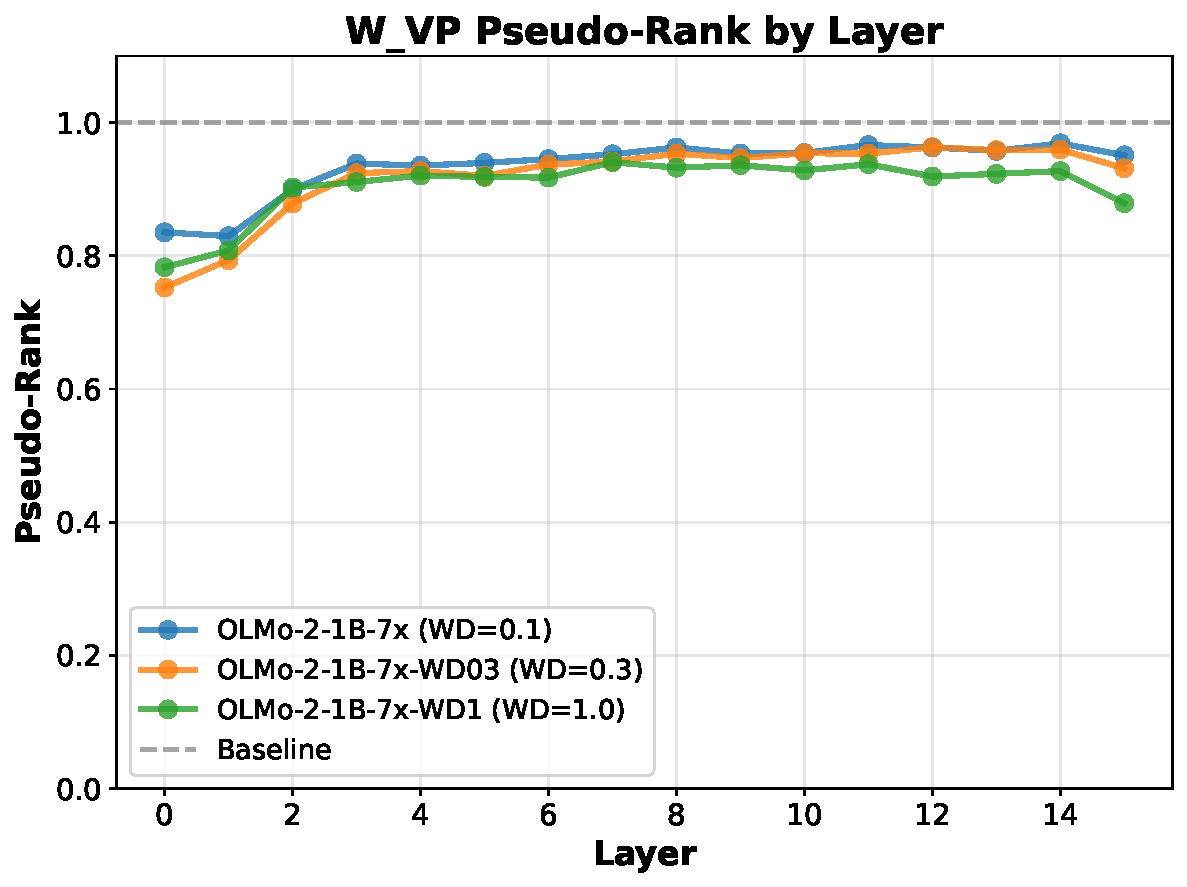
\includegraphics[width=\linewidth]{figs/rank_attn_matrices/olmo2_1b_7x_weight_decay_comparison_vp.pdf} 
        \caption{Value-Projection}
    \end{subfigure}
    \caption{{\bf Weight decay reduces the rank of attention matrices.} This is for the OLMo models trained at 140 TPP. We observe that the rank of attention for weight decay 0.1 is generally smaller than that for both the 20 TPP and the fully trained OLMo-2-1B-0425 model. Hence, we conjecture that this is because the 140 TPP models were trained with a warmup-stable-decay learning rate schedule, whereas the 1x and 144x models were trained with a cosine learning rate schedule. While it has been shown that WSD leads to a similar validation loss to cosine decay \citep{hagele2024scaling}, there is emerging evidence that there are important differences between the training dynamics of the two learning rate schedules \citep{catalan2025training}.}
\end{figure*}

\begin{figure*}[h] 
    \centering
    \begin{subfigure}[b]{0.24\textwidth} 
        \centering
        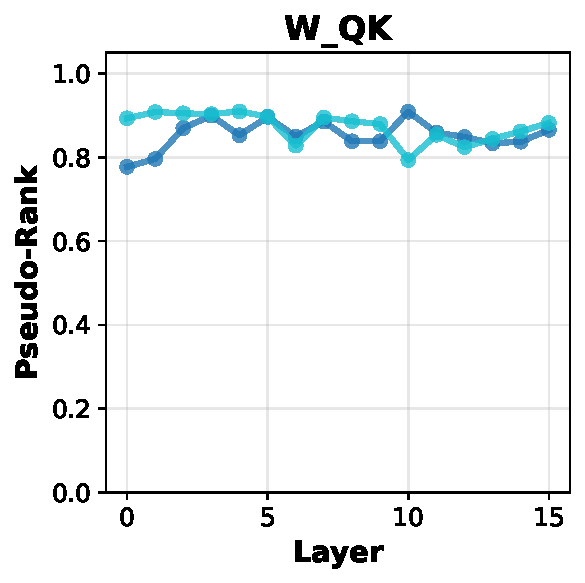
\includegraphics[width=\linewidth]{figs/rank_attn_matrices/olmo_by_layer_qk.pdf} 
        \caption{Query-Key}
    \end{subfigure}
    \begin{subfigure}[b]{0.24\textwidth} 
        \centering
        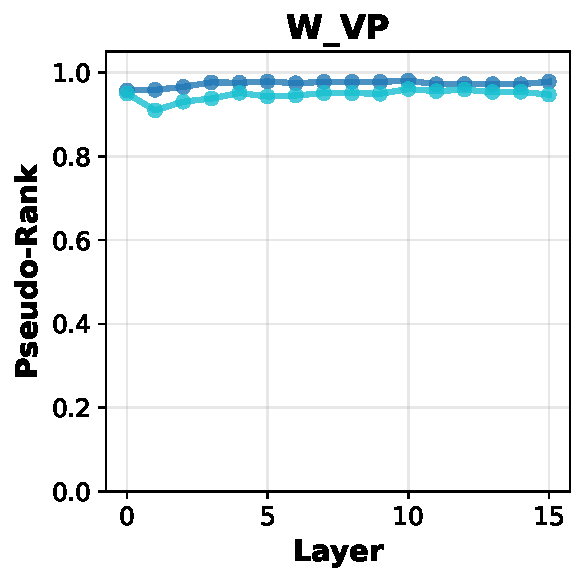
\includegraphics[width=\linewidth]{figs/rank_attn_matrices/olmo_by_layer_vp.pdf} 
        \caption{Value-Projection}
    \end{subfigure}$\,$\\[4pt]

\includegraphics[width=0.4\textwidth]{figs/rank_attn_matrices/olmo_by_layer_legend.pdf}
    \caption{{\bf Training time does not reduce the rank of attention matrices.}  }
    \label{fig:attention_rank_training_time}
\end{figure*}





\begin{figure*}[h]
    \centering
    \begin{subfigure}[b]{0.3\textwidth} 
        \centering
        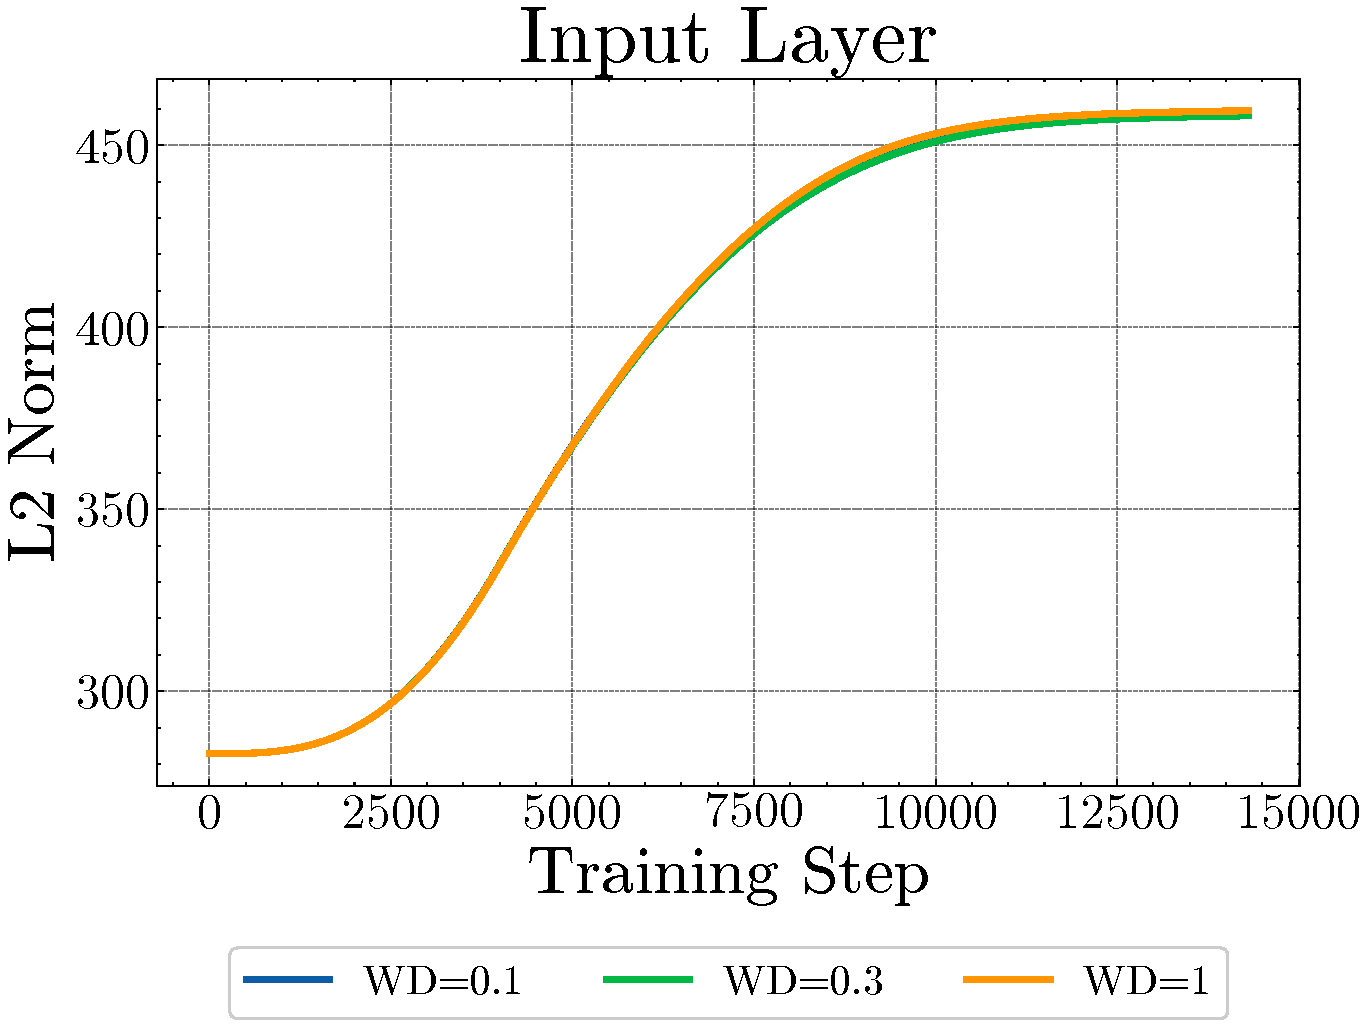
\includegraphics[width=\linewidth]{figs/rank_attn_matrices/wd_ablation_1x_input_layer.pdf} 
        \caption{Input Layer}
    \end{subfigure}
    \hfill
    \begin{subfigure}[b]{0.3\textwidth} 
        \centering
        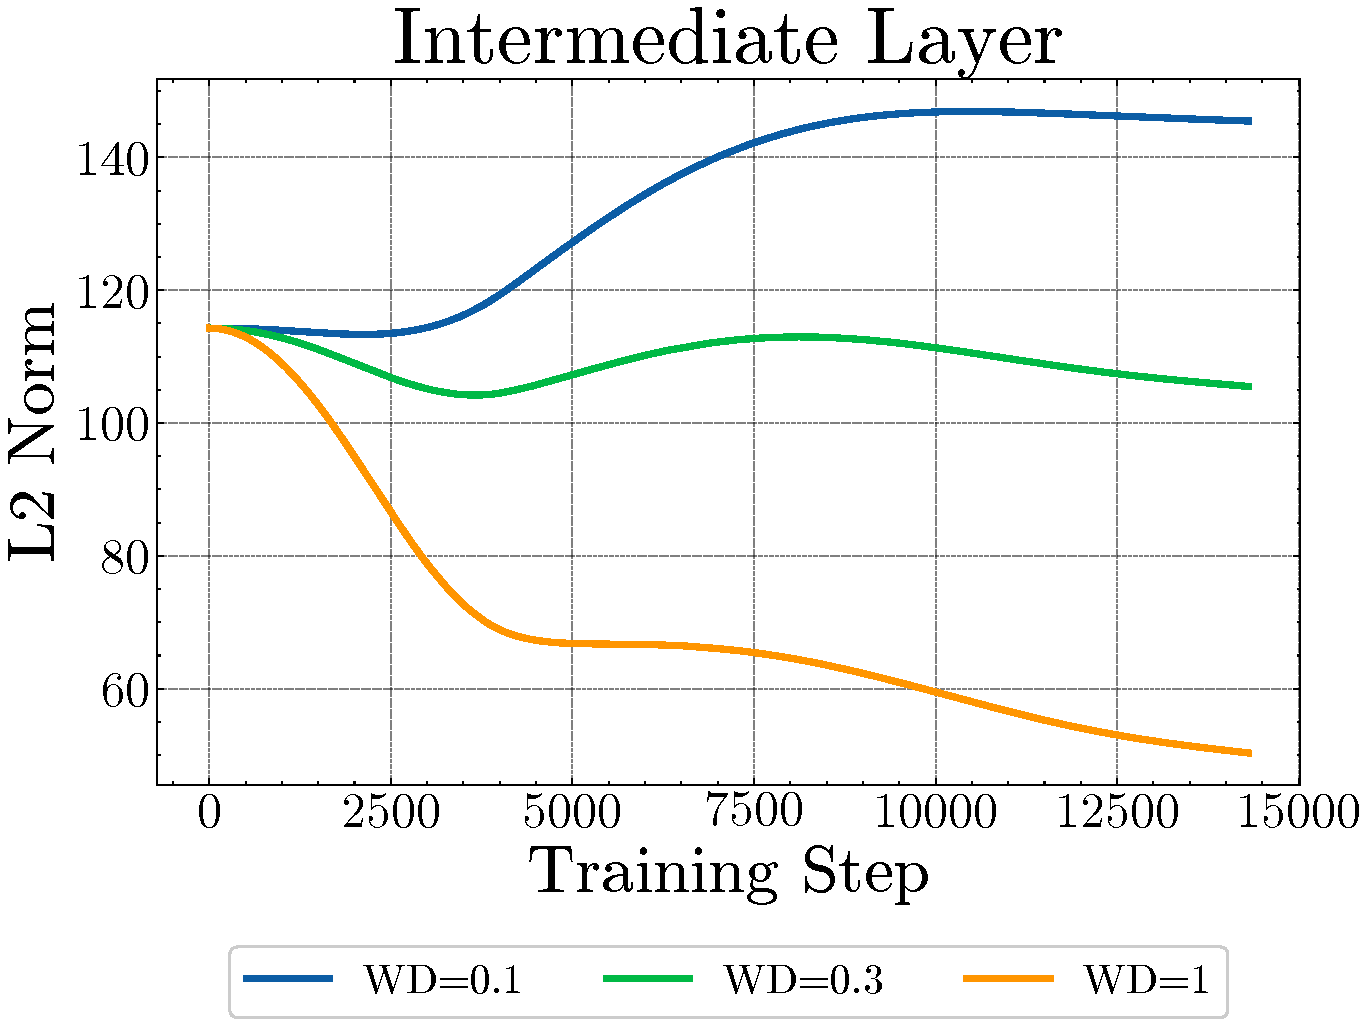
\includegraphics[width=\linewidth]{figs/rank_attn_matrices/wd_ablation_1x_intermediate_layer.pdf} 
        \caption{Intermediate Layer}
    \end{subfigure}
    \hfill
    \begin{subfigure}[b]{0.3\textwidth} 
        \centering
        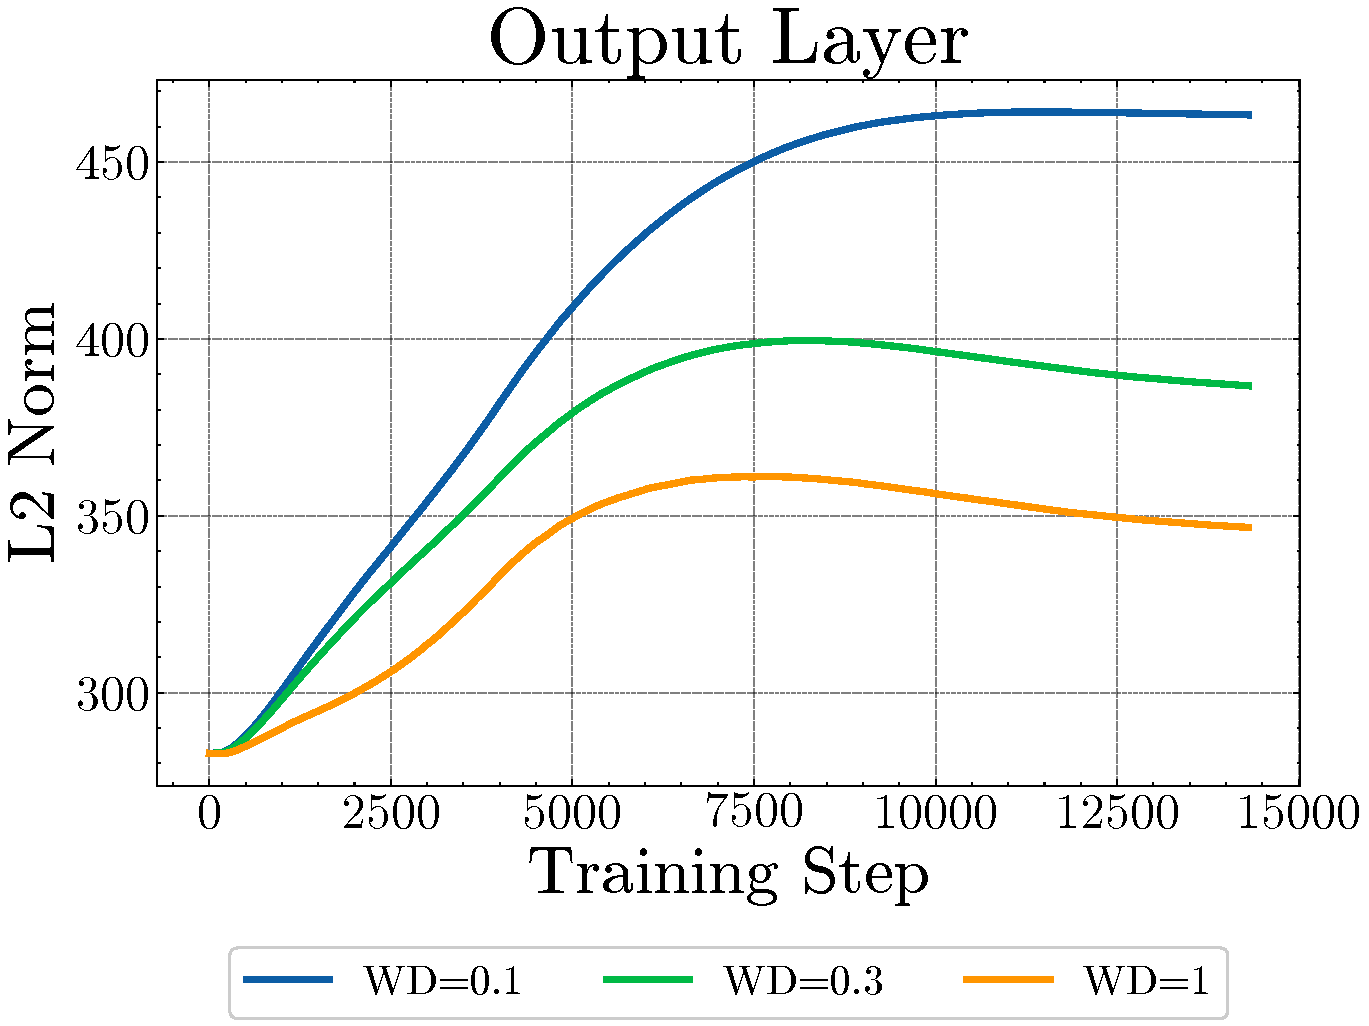
\includegraphics[width=\linewidth]{figs/rank_attn_matrices/wd_ablation_1x_output_layer.pdf} 
        \caption{Output Layer}
    \end{subfigure}
    \caption{{\bf Weight decay reduces the norm of the weights of the model.} The effect does not occur for the input layer, where the weights are not being decayed. This is for OLMo-2-1B models trained at 20 TPP.  }
\end{figure*}


\clearpage
\subsection{Norm of parameters}

We also examine how weight decay changes the distribution of parameter norms across layers (Figure~\ref{fig:app-parameter-norms}). The parameter norm of intermediate layers as a fraction of total model norm slightly decreases as weight decay increases. This is because the relative norm of lm\_head (and the embedding layer which is not weight decayed for OLMo models) grows.


\begin{center}
    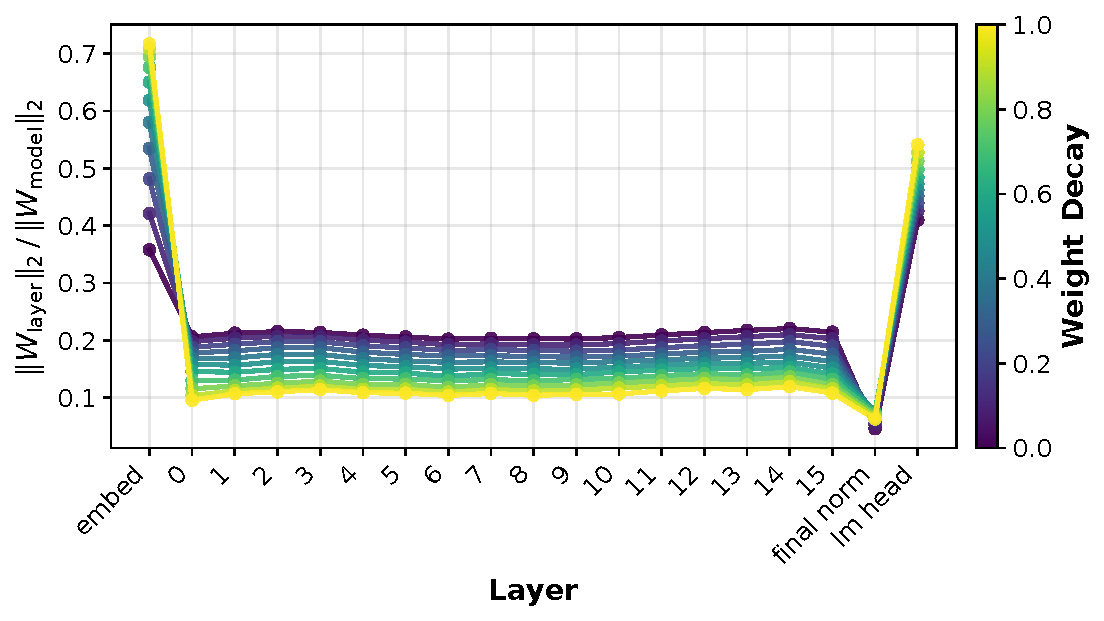
\includegraphics[width=0.6\linewidth]{figs/parameter_norm/olmo_2_1b_1x_wd_ablation_layer_norm_fraction.pdf}
    \captionof{figure}{{\bf Effect of weight decay on parameter norm.} The figure depicts the per-layer L2-norm fraction for the \olmoonex{} models. The depicted layer-wise values are the sum of all of the layers parameters.}
    \label{fig:app-parameter-norms}
\end{center}